\chapter{Arduino}

%BRIDGE FROM PREVIOUS SECTION
The Arduino Uno in this project acts as a bridge between hardware and software, allowing the navigation stack on the laptop to read sensor data from the rover, and control the speed of its wheels.

\section{Background}
Arduino development boards are printed circuit boards (PCBs) with an on-board microcontroller, timing crystal, USB port, I/O pins and more. The board used in this project, an Arduino Uno, uses the ATmega328P microcontroller with a 16 MHz quartz timing crystal and has 14 digital I/O pins. It also has 6 analog I/O pins, but we won't make use of them in this project. 

Digital I/O pins can be configured to either read signals as input or generate them as output. Digital pins read input signals at specific times as binary values, that is the connected signal's voltage is read as either LOW or HIGH. They are also capable of generating binary output voltage, HIGH and LOW signals.

\subsection{Servo Control Pulses} \label{sectionRCPulses}
An important use-case which pops up often when using the Arduino is that of interfacing with RC electronics. In this project's design, both the Sabertooth motor driver and the standard servo require their signal inputs to use the standard R/C transmission protocol. In fact, the standard servo contains among other components an internal motor driver, and so 

This protocol involves sending brief pulses of a HIGH signal, between one and two milliseconds. There is a fixed delay between pulses, commonly about 20 ms of LOW signal. The width of the HIGH pulse communicates to a servo the desired position. Its internal components then drive its DC motors until the servo is rotated to the commanded position. In the case of the Sabertooth motor driver, the position is interpreted as a speed to drive the motors at.

\section{Arduino Uno Connections}
Refer back to Figure \ref{figRoverDesign} for a visual representation of how the Arduino Uno is connected to the other rover components.

\subsection{Hardware Interrupt Pins} \label{sectionHIP}
As one can see in Figure \ref{figRoverDesign}, only two optical quadrature encoders are used, with one placed on the front motor for both the left and right side of the rover. This is due to a hardware limitation of the Arduino Uno. The ATmega328P microcontroller has only two interrupt pins, which are mapped to digital pins 2 and 3 on the Uno. These pins can trigger unique Interrupt Service Routines (ISRs) whenever the input signals change from LOW to HIGH voltage, or vice versa.

While it is possible to create interrupts which react to a change in a pin's voltage for any digital pin, these will be slower than ISRs from hardware interrupts. A hardware interrupt is necessary to keep up with the fast rate of pin voltage changes that occur in the output of quadrature encoders.

If a different Arduino board such as the Mega were used, there would be sufficient hardware interrupt pins for all four encoders. Using a board with plentiful interrupts, one could even attach both channel outputs of the encoders to interrupt pins, rather than only one. This would double the encoders' resolution \cite{encoderBlog}.

\subsection{Digital Pin Connections}
Each motor encoder has two output channels, channel A and channel B. Both encoders attach one of their output channels, channel A, to a hardware interrupt pin. In section \ref{sectionQuadEncoders} we will see why this configuration was chosen. The right motor's encoder connects channel A to pin 2, and channel B to pin 4. The left motor's encoder connects its channel A output to pin 3, and its channel B output to pin 7. 

The S1 and S2 signal input terminals on the Sabertooth motor driver are connected to digital pins 5 and 6. The control signal for the hobby servo is connected to digital pin 9. The signal pin on the ultrasonic sensor is connected to digital pin 11. The Arduino's ground pin is connected to the ground of the motor driver's BEC, to ensure a common ground plane.

Most digital pin numbers used are arbitrary, and connections may be permuted without issue. The exceptions are pins 0-3, which must not be modified. Pins 0 and 1 must be left unattached for serial data transfer to work properly over USB. And pins 2 and 3 are hardware interrupt pins which must be used to handle the quadrature encoders' output.

\section{Motor Driver's Configuration}
The Sabertooth motor driver has two signal input terminals, S1 and S2, which allow the Arduino to issue instructions specifying how to drive the motors. The protocols used to communicate with the motor driver over these signal inputs are specified by DIP switches on-board the driver. There are six of these DIP switches, and they can be flipped either up or down.

Setting switch 1 down and switch 2 up places the driver into R/C input mode, which configures S1 and S2 to expect servo control pulses, à la R/C controllers. This protocol was briefly explained in section \ref{sectionRCPulses}. \cite{sabertoothUserGuide}

Turning switch 3 down selects the lithium cutoff mode, which detects the number of lithium cells in series powering the driver, and shuts off when the battery pack's voltage drops below 3.0V per cell, or 6.0V for the two cell battery pack this project uses. This prevents accidental damage to the 18650 cells which may be caused by over-discharge.

Flipping switch 4 down selects independent (differential) drive, which allows S1 and S2 to each independently control the speed of one motor channel. Using this mode, turning of the vehicle is achieved by lowering the relative speed of the motors on one side of the vehicle compared to the other.

Switch 5 is flipped up to ensure a linear rather than exponential response of the motors to the Arduino's input signal. Switch 6 is flipped down to select "microcontroller mode", which turns off auto-calibration of the zero-velocity input signal, and turns off an automatic timeout. Thus if the signal connection is somehow lost the motor driver will continue driving the motors according to the last signal received. This is necessary for smooth performance of the motors since the Arduino may slightly delay control pulses. Though this introduces a risk of loss of control should wires come disconnected, it is a small one that should only occur during a catastrophic crash.

\section{Arduino Sketch}
A sketch is Arduino-speak for an embedded program written for an Arduino board. There is an Arduino IDE which supports development of sketches in C or C++, and allows one to take advantage of a software library for common I/O interactions. After the code is written in this IDE, it is uploaded to the board over a USB serial connection. The board will then continuously execute the code found in the sketch's main loop as long as the board is powered. This embedded software interacts with the various sensors and other electronics on a low level, through reading from and writing to the Arduino's digital I/O pins.

Part of the standard Arduino library is the Servo library. This library allows one to configure a digital pin to output RC control pulses, as explained in section \ref{sectionRCPulses}. The sketch used in this project uses this library to specify the speed of each set of wheels driven by the Sabertooth motor driver, and to control the position of the standard servo aiming the ultrasonic range sensor.

%\lstinputlisting[language=C++]{../AutoRover/Arduino/rover_sketch/rover_sketch.ino}

\subsection{Quadrature Encoders} \label{sectionQuadEncoders}
An important function of the Arduino sketch is to track the movement of the motors. Our system may command the motor driver to move the rover's wheels with a certain fraction of the maximum available power, but it is difficult to predict with precision the resulting angular velocity. For one thing, the RPM of DC motors is proportional to the supplied voltage. But the voltage supplied to the motors through the motor driver is coming from an external li-po battery pack, which generates variable voltage. It starts at 8.4V and drops to a minimum of 6.0V before the motor driver shuts off. Thus even if the same servo control pulse is continuously sent to the motor driver, the motors' angular velocity will decrease over time.

In order to determine the true angular velocity of the motors, rotary encoders are attached to them. These feedback devices are incremental position encoders, meaning they monitor the change in the motor shaft's position compared to some starting position. 

\begin{wrapfigure}{l}{0.5\textwidth}
	\caption{\cite{fig_optical_encoders}}
	\centering
	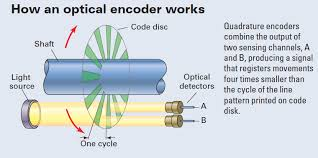
\includegraphics[width=0.5\textwidth]{opticalEncoders}
	\label{FigOpticalEncoders}
\end{wrapfigure}

The motor encoders which came with the Lynxmotion rover kit are optical quadrature encoders. This type of encoder attaches a flat disk with thin slits known as the code disk to the motor's gear shaft. Two photodiodes, components which transform light into electric current, are placed above the disk side by side. A light source shines light through the disk from the other side. See Figure \ref{FigOpticalEncoders} for a visual illustration.

As the motor spins the gear shaft, the code disk turns with it. This produces an on-off pattern of light on the photodiodes, which produce two square waves as signal outputs. These two channels of output pulses are referred to as channels A and B. Depending on the direction of rotation, channel A's square wave will either lag behind or be ahead of channel B. This can be seen in Figure \ref{FigQuadChannels} which shows example output pulses as a motor turns clockwise (CW) or counter-clockwise (CCW). \cite{encoderBlog}

The number of slits in the code disk corresponds directly to how many pulses each channel will produce in one revolution of the DC motor. This is known as the pulses per revolution (PPR), and is given by the manufacturer. By counting how many pulses occur in one second, and using the PPR, one can calculate the angular speed of the motor. If one wishes for greater resolution, they can watch each square wave for a change in voltage from LOW to HIGH or HIGH to LOW. This gives a maximum resolution of \(4 * PPR\) detectable position increments per revolution.

\begin{figure}[h]
	\caption{\cite{fig_quad_channels}}
	\centering
	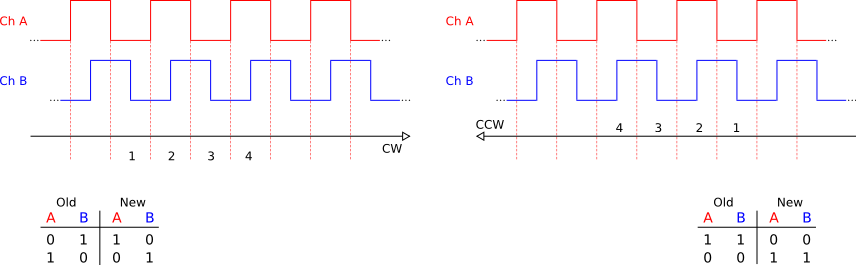
\includegraphics[width=\textwidth]{quadrature}
	\label{FigQuadChannels}
\end{figure}

Handling rapid changes in voltage is exactly what hardware interrupts are designed for. Unfortunately, for maximum resolution each encoder needs two hardware interrupt pins, one for each channel. The Arduino Uno only has two hardware interrupt pins, and our rover has two sides. It would be nice if we could at least use two encoders, one for each side.

We achieve this by reacting to changes in voltage in only one channel per encoder. In the two tables in Figure \ref{FigQuadChannels}, LOW voltage values are encoded as 0, and HIGH voltage values as 1. The first plot in the figure shows the output of the two channels when the motor is moving in the CW direction.  When channel A transitions from the section labeled 1 to section 2, it is rising from 0 to 1, and channel B has value 0. That information alone tells us that the motor's gear shaft is turning, but not in what direction. However, at the next transition between sections 2 and 3, channel A falls from 1 to 0, and channel B has value 1. Now we are confident that channel B began its pulse after channel A. This means that the photodiode generating channel B detected light after channel A's photodiode, i.e. the code disk is turning in the direction of photodiode A to B. Datasheet specifications will tell us that this translates to the CW direction. It turns out that for each channel A transition event, the previous and new channel values are sufficient to uniquely determine the direction of rotation of the motor. Thus, while only monitoring one of the channels lowers our resolution to \(2 * PPR\) counts per revolution, it allows us to use hardware interrupts for two quadrature encoders rather than only one. \cite{encoderBlog}

The sketch uses an implementation described in \cite{encoderBlog}, which creates a lookup table using the four binary digits representing the previous and current channel states. These digits form a four-bit binary number, which indexes into a sixteen element array. Each element of this array stores either 1, -1, or 0, where 1 represents a movement in the CW direction, -1 represents a movement in the CCW direction, and 0 represents an indeterminate transition. This lookup table is then used by the sketch when it reacts to a hardware interrupt caused by the channel A output of one of the encoders. When this interrupt occurs, the code reads the values of channels A and B from the corresponding digital pins, and combines them with the previous values to find the appropriate index in the lookup table. The value at that index is then added to a global counter variable, which keeps track of the net number of incremental movements from the motor's starting position. A net negative number indicates how far the motor has rotated in the CCW direction since it started, and a net positive number indicates how far the motor has rotated in the CW direction. \cite{encoderBlog}



% TODO: BELOW
TODO TODO TODO
TODO TODO TODO
text in this chapter below this line is not finished

When one of the digital pins connected to Channel A change, the main loop of the sketch is interrupted, and the corresponding interrupt service routine (ISR) is executed. Until this ISR finishes, no other code is run, including other interrupt events, though they may be flagged for future execution. Therefore ISRs must be as fast as possible, to not cause any interrupt events to be dropped, and to ensure that the main loop continues running smoothly.

PIND returns input readings from pins 0-7 as a byte.
The below code uses bit shifting and masking to put
the values of digital input pins 4 (output B) and 
2 (output A) into the least significant bit and 
second-least significant bit of the enc\_val 
variable, respectively.

\begin{mdframed}[backgroundcolor=light-gray, roundcorner=10pt,leftmargin=1, rightmargin=1, innerleftmargin=15, innertopmargin=15,innerbottommargin=15, outerlinewidth=1, linecolor=light-gray]
\begin{lstlisting}[language=C++]
volatile long encLeftCount = 0L;
const int8_t encoder_lookup_table[] =
    {0,0,0,-1,0,0,1,0,0,1,0,0,-1,0,0,0};
void encoderLeft_isr() {
static uint8_t enc_val = 0;
enc_val = enc_val << 2; // Store the previous 2-bit code
enc_val = enc_val | ( ((PIND & 0b100) >> 1) |
    ((PIND & 0b10000) >> 4) );
encLeftCount = encLeftCount + 
    encoder_lookup_table[enc_val & 0b1111];
}
\end{lstlisting}
\end{mdframed}

\subsection{Timing}
The serial communication between the Arduino and laptop is setup at a baud rate (equivalent to bit rate per second) of 115,200. The USB connection between the Arduino and laptop uses a cable supporting a data transfer rate of 480 Mbps (480 million bits per second). Ten bits are used per byte sent over the serial port (one start bit, 8 data bits, one stop bit), so 480 Mbps / 10 bits = 48 MBps. Let’s calculate the maximum data transfer rate I will need for all my sensors + motor commands (should be much less than 53 MBps).

The Arduino Uno has 3 timers, timer0, timer1, timer2. Timer0 controls millis() and delay() in Arduino. Timer1 is used by the Servo library. Timer2 is used by the NewPing library.

Each encoder generates 100 pulses per revolution. We will only be watching one of the square waves (output channel A), so that’s 200 edge transitions per revolution. The motors are 200 rpm, so at maximum speed the two motors with encoders attached would see less than 3.4 revolutions per second. So there will be at most 3.4 * 200 = 680 counts per second. So there will be at least 1 sec / 680 =~ 1.4 milli seconds between counts.
9600 baud = 960 bytes / sec is more than enough for (14 byte per sensor update) * (30 updates per second (limit on ultrasonic sensor)) = 420 bytes per sec. At 960 bytes/sec, there is about a millisecond between byte transmissions. 

Interrupt guards have been placed around code copying two long encoder counting variables (4 bytes) that are modified within ISRs. Each assignment to a local temp variable should translate to 4 machine instructions, so there will be 8 machine instructions between interrupt guards. The Arduino Uno uses a 16 MHz quartz crystal, so it can process 16 million instructions per second, which means it takes 1 sec / 16 million instructions = 6.25e-8 of a second per instruction. Thus to run the 8 instructions inside the guard takes 8 * 6.25e-8 = 5e-7 or half a micro second. 

The worst case scenario would be for all possible interrupts to flag their events (serial RX, two hardware pins for quadrature encoders, plus Arduino background interrupts like the one for millis) right after interrupt handling is disabled. In this case, as long as interrupts are enabled and handled before another interrupt event occurs, no events will be lost. External interrupt calling has an overhead of 5.125 microseconds (5.125e-6), and each ISR should not take many microseconds \cite{gammonInterrupts}. Thus the interrupt guards should not cause a problem for either the 1400 micro seconds of time until the next possible quadrature encoder pin change or for the 1000 micro seconds until the next incoming serial byte. After exiting the interrupt guard, all interrupts are guaranteed to be handled before the next event arrives.

\subsection{Ultrasonic Sensor}
The PING))) ultrasonic distance sensor works by emitting a short burst of 40 kHz sound waves and timing the delay before an echo response. The Arduino triggers a ping by generating a brief 5 \(\mu\)s pulse on the sensor's bi-directional signal pin. The sensor then generates a HIGH output pulse, which continues until either the echo is received or the maximum amount of time, 18.5 ms, has passed. This time may then be multiplied by the speed of sound in air to calculate an estimated distance of the first object in front of the sensor. \cite{pingDocumentation}

The sketch uses the NewPing library to handle this protocol \cite{newPing}. This library provides a convenient method, ping() which returns the echo time in \(\mu\)s. The sketch reports this time rather than a distance, since the speed of sound in air depends on the current air temperature. The appropriate conversion is made by the repeater node on the laptop, see section \ref{RepeaterNode}.

\subsection{Servo}
The ultrasonic sensor can only detect objects which are roughly straight in front of it. Thus for the rover to have a greater view of its surroundings, the sensor needs to be panned back and forth, to "look" straight ahead, left, and right. This is what the standard servo it is attached to allows. The sketch makes use of the standard Servo library to control the servo with PPM signals. An angular degree from 0 to 180 is written to a Servo object, and the servo library handles generating the output signal for the digital pin corresponding to that object.

The sketch sweeps the servo back and forth one degree at a time, and at each step a range reading (in \(\mu\)s) from the PING))) sensor is taken. This reading, along with the servo's position in degrees, and the current motor encoder values, are then transmitted over serial.

This is shown in the following code for an arbitrary step size:
\begin{mdframed}[backgroundcolor=light-gray, roundcorner=10pt,leftmargin=1, rightmargin=1, innerleftmargin=15, innertopmargin=15,innerbottommargin=15, outerlinewidth=1, linecolor=light-gray]
\begin{lstlisting}[language=C++]
void setup() {
sonicServo.attach(sonicServoPin);
sonicServo.write(SERVO_RIGHT);
}
void loop() {
servoPos = SERVO_RIGHT; // initial servo position
while (servoPos < SERVO_LEFT) {
sonicServo.write(servoPos);
delay(SERVO_STEP_DELAY); 
ping_time_uS = sonar.ping();
pushSensorUpdate(servoPos, ping_time_uS);
servoPos = min(servoPos + SERVO_STEP_SZ, SERVO_LEFT);
}
while (servoPos > SERVO_RIGHT) {
sonicServo.write(servoPos);
delay(SERVO_STEP_DELAY); 
ping_time_uS = sonar.ping(); 
pushSensorUpdate(servoPos, ping_time_uS);
servoPos = max(servoPos - SERVO_STEP_SZ, SERVO_RIGHT);
}
}
\end{lstlisting}
\end{mdframed}


\subsection{Communication Protocol}
Serial communication over usb
Hexadecimal ASCII - why?
sends ping time, servo position, and both encoders tick counts at each servo position when it stops to take a range reading. This occurs at roughly 20 Hz.

receives instructions, sets channel 1 and 2 accordingly


* Reading from multi-byte variables which are accessed within
* and without an ISR risks data corruption, so interrupt guards
* must be used around a read to make it atomic.

// worst case scenario, two encoder interrupt flags and serial RX flag are set right after noInterrupts();

long is 4 bytes, so assignment translates to 4 machine instructions.

// turn all interrupts back on, run next statement, then handle any that were flagged in-between guards
\begin{mdframed}[backgroundcolor=light-gray, roundcorner=10pt,leftmargin=1, rightmargin=1, innerleftmargin=15, innertopmargin=15,innerbottommargin=15, outerlinewidth=1, linecolor=light-gray]
	\begin{lstlisting}[language=C++]
noInterrupts(); // turn off all interrupts
encLeftCount_temp = encLeftCount;
encRightCount_temp = encRightCount;
interrupts(); // turn all interrupts back on
	\end{lstlisting}
\end{mdframed}

Send sensor data to processing unit over serial port, with descriptive start bytes.
None of the start bytes should be in the range '0' - '9' or 'a' - 'f', since those 
chars are used by the hexadecimal ASCII encoding.
L == Left motor's quadrature encoder's position value
R == Right motor's quadrature encoder's position value
S == Angular degree of servo
P == Ultrasonic ping time (in micro seconds) measured at the given servo angle